% fix a0poster for compilation with lualatex
% https://tex.stackexchange.com/a/411473
\RequirePackage{luatex85}
\RequirePackage{shellesc}
\newcount\pdfshellescape
\pdfshellescape=1 % unrestricted shell-escape

\documentclass[a0,portrait]{a0poster}


% TU DORTMUND-LIKE FONT
\usepackage[no-math]{fontspec}
\setsansfont[
    Ligatures = TeX,
    BoldFont = FiraSans,
    ItalicFont = FiraSans-LightItalic,
    BoldItalicFont = FiraSans-Italic,
    FontFace = {bxx}{n}{FiraSans-SemiBold}
]{FiraSans-Light}
\newcommand{\bxseries}{\fontseries{bxx}\selectfont}
% \usefonttheme[onlymath]{serif}

% TIKZ
\usepackage[pdftex]{graphicx,color}
\DeclareGraphicsExtensions{%
    .pdf,.PDF,%
    .png,.PNG,%
    .jpg,.jpeg,.JPG,.JPEG}
\usepackage{tikz}
\usepackage{pgfplots}
\pgfplotsset{compat=1.15}
\usetikzlibrary{calc,patterns,shapes,positioning,arrows.meta}
\usetikzlibrary{decorations.pathreplacing}
\usepgfplotslibrary{fillbetween}



% COLOR PALETTE
\usepackage{ifthen}
\newcommand{\colorpalette}[1]{%

	% color palette by Erich Schubert https://bitbucket.org/ls8-tudo/beamer-erich/src/template/
	\xdefinecolor{tugreen}{RGB}{132, 184, 24} % source: official
	\xdefinecolor{tudarkgreen}{RGB}{100, 150, 0} % source: official (purpose: web design)
	\xdefinecolor{tulightgreen}{RGB}{224, 234, 204} % source: official (purpose: web design)
	\xdefinecolor{tugray}{RGB}{207, 208, 210} % source: Powerpoint template diagram
	\xdefinecolor{tugraybg}{RGB}{178, 179, 204} % source: official (purpose: web design)
	\xdefinecolor{tuorange}{RGB}{227, 105, 19} % source: another template
	\xdefinecolor{tuyellow}{RGB}{242, 189, 0} % source: another template
	\xdefinecolor{tucitron}{RGB}{249, 219, 0} % source: another template
	\xdefinecolor{tublue}{RGB}{46, 134, 171} % source: imaginary
	\xdefinecolor{tudarkblue}{RGB}{30, 89, 114} % source: imaginary
	\xdefinecolor{tuviolet}{RGB}{61, 52, 139} % source: imaginary
	\xdefinecolor{tumagenta}{RGB}{139, 52, 88} % source: imaginary
	\xdefinecolor{tudarkergreen}{RGB}{75, 98, 44} % source: Stefan Michaelis
	\xdefinecolor{tuolive}{RGB}{83, 145, 45} % source: Stefan Michaelis
	\xdefinecolor{tulime}{RGB}{215, 215, 0} % source: Stefan Michaelis
	\xdefinecolor{tugraygreen}{RGB}{217,233,229} % source: Stefan Michaelis

	% ML2R colors
	\xdefinecolor{ml2rteal}{RGB}{0, 147, 145} % source: Powerpoint ML2R template
	\xdefinecolor{ml2rblue}{RGB}{1, 105, 140} % source: Powerpoint ML2R template
	\xdefinecolor{ml2rorange}{RGB}{250, 184, 47} % source: Powerpoint ML2R template
	\xdefinecolor{ml2rgreen}{RGB}{128, 181, 44} % source: Powerpoint ML2R template

	% gray tones
	\colorlet{lightgray}{gray!25}
	\colorlet{midlightgray}{gray!60}
	\colorlet{anthracite}{black!85}

	% switch between 'tu' and 'ml2r'
	\ifthenelse{\equal{#1}{tu}}{%
		\colorlet{tu01}{tugreen}
		\colorlet{tu02}{tuorange}
		\colorlet{tu03}{tuyellow}
		\colorlet{tu04}{tucitron}
		\colorlet{tu05}{tublue}
		\colorlet{tu08}{tuviolet}
		\colorlet{tu06}{tumagenta}
		\colorlet{tu07}{tuolive}
		\colorlet{tu09}{tulime}
		\colorlet{tu10}{tudarkblue}
		\colorlet{tu11}{tugraygreen}
	}{\ifthenelse{\equal{#1}{ml2r}}{%
		\colorlet{tu01}{ml2rgreen}
		\colorlet{tu02}{ml2rorange}
		\colorlet{tu03}{ml2rteal}
		\colorlet{tu04}{ml2rblue}
		\colorlet{tu05}{tuorange}
		\colorlet{tu06}{tumagenta}
		\colorlet{tu07}{tugraybg}
		\colorlet{tu08}{tuviolet}
		\colorlet{tu09}{tudarkgreen}
		\colorlet{tu10}{tudarkblue}
		\colorlet{tu11}{tulightgreen}
	}{%
		\GenericError{}{Error: \string\palette\space requires argument 'tu' or 'ml2r'}{}{}
	}}

	% mixed colors
	\colorlet{tu01light}{tu01!40}
	\colorlet{tu02light}{tu02!40}
	\colorlet{tu03light}{tu03!40}
	\colorlet{tu04light}{tu04!40}
	\colorlet{tu05light}{tu05!40}
	\colorlet{tu06light}{tu06!40}
	\colorlet{tu07light}{tu07!40}
	\colorlet{tu08light}{tu08!40}
	\colorlet{tu09light}{tu09!40}
	\colorlet{tu10light}{tu10!40}
	\colorlet{tu11light}{tu11!40}

	\colorlet{tu01midlight}{tu01!60}
	\colorlet{tu02midlight}{tu02!60}
	\colorlet{tu03midlight}{tu03!60}
	\colorlet{tu04midlight}{tu04!60}
	\colorlet{tu05midlight}{tu05!60}
	\colorlet{tu06midlight}{tu06!60}
	\colorlet{tu07midlight}{tu07!60}
	\colorlet{tu08midlight}{tu08!60}
	\colorlet{tu09midlight}{tu09!60}
	\colorlet{tu10midlight}{tu10!60}
	\colorlet{tu11midlight}{tu11!60}

	\colorlet{tu01dark}{tu01!80!black}
	\colorlet{tu02dark}{tu02!80!black}
	\colorlet{tu03dark}{tu03!80!black}
	\colorlet{tu04dark}{tu04!80!black}
	\colorlet{tu05dark}{tu05!80!black}
	\colorlet{tu06dark}{tu06!80!black}
	\colorlet{tu07dark}{tu07!80!black}
	\colorlet{tu08dark}{tu08!80!black}
	\colorlet{tu09dark}{tu09!80!black}
	\colorlet{tu10dark}{tu10!80!black}
	\colorlet{tu11dark}{tu11!80!black}

	\colorlet{tu01middark}{tu01!90!black}
	\colorlet{tu02middark}{tu02!90!black}
	\colorlet{tu03middark}{tu03!90!black}
	\colorlet{tu04middark}{tu04!90!black}
	\colorlet{tu05middark}{tu05!90!black}
	\colorlet{tu06middark}{tu06!90!black}
	\colorlet{tu07middark}{tu07!90!black}
	\colorlet{tu08middark}{tu08!90!black}
	\colorlet{tu09middark}{tu09!90!black}
	\colorlet{tu10middark}{tu10!90!black}
	\colorlet{tu11middark}{tu11!90!black}
}

\colorpalette{tu} % OR: \colorpalette{ml2r}



% COLUMNS
\usepackage{multicol}
\columnsep=16mm      % white space between columns
\columnseprule=0pt    % thickness of line between columns
% \renewcommand{\columnseprulecolor}{\color{gray}}

% ENUMERATIONS
\usepackage{enumitem}
\newcommand*\tubullet{%
    \begin{tikzpicture}
        \draw[ultra thick, gray, fill=tu01] (0, 0) circle[radius=5pt];
    \end{tikzpicture}
}
\setlist{%
    labelindent=0pt,
    labelwidth=*,
    labelsep*=6mm,
    itemindent=0cm,
    leftmargin=!,
    topsep=0pt,
    font={\bfseries\sffamily\normalsize}
}
\setlist[itemize]{label=\raisebox{4pt}{\protect\tubullet}}
\setlist[description]{itemsep=\parskip}

% BOX LAYOUT
\newcommand{\resettikz}{\tikzset{every node/.style={text width=, minimum width=0pt, inner sep=10pt, font=\normalsize}, every path/.style={thick}}} % do not inherit
\newcommand{\resetfont}{\sffamily\normalsize}
\newcommand{\plainsection}[1]{\resetfont\noindent\begin{center}\bfseries\Large#1\end{center}\vspace*{2mm}}
\newcommand{\plainsubsection}[1]{\resetfont\noindent{\bfseries\large#1}}

\usepackage{etoolbox} % provides \patchcmd
\renewcommand{\refname}{References}
\patchcmd{\thebibliography}{\section*}{\plainsection}{}{}

\renewcommand{\section}[2][tu01]{%
    \noindent
    \begin{tikzpicture}
        \node[white,
            fill = #1,
            draw = none,
            rounded corners = 12pt,
            minimum width = \columnwidth,
            inner xsep = 0pt,
            inner ysep = 5pt,
            outer sep = 0pt,
            text height = 14mm,
            text width = .85\columnwidth,
            align = center,
            use as bounding box] (title) at (0,0) {\resetfont\bfseries\Large #2\strut};
        \fill[#1] ($(title.south west) + (0pt,12pt)$) -- ++(0pt,-12pt) -- ++(12pt,0pt) -- cycle;
        \fill[#1] ($(title.south east) + (0pt,12pt)$) -- ++(0pt,-12pt) -- ++(-12pt,0pt) -- cycle;
    \end{tikzpicture}%
}

\usepackage{environ} % provides the \NewEnviron command for custom environments

% basic implementation of the sectionbox and sectionbox* environments (see below)
\NewEnviron{innersectionbox}[2][tu01]{%
    \noindent
    \begin{minipage}{\columnwidth}
        \section[#1]{#2}
        \vskip -2pt % perfect alignment (if different colors are used for the heading and the box) with -2.025pt
        \noindent
        \begin{tikzpicture}
            \node[minimum width = \columnwidth,
                text width = .85\columnwidth,
                text justified,
                inner sep = 20pt,
                outer sep = 0pt,
                use as bounding box] (body) at (0,0) {\resettikz\resetfont\setlength{\parskip}{9mm}\vspace*{-9mm}\par\BODY};
            \draw[#1midlight,
                line width = 2pt,
                rounded corners = 12pt] ($(body.north west) + ( 1pt,0pt)$) -- ($(body.south west) + ( 1pt,-6mm)$) --
            ($(body.south east) + (-1pt,-6mm)$) -- ($(body.north east) + (-1pt,0pt)$);
        \end{tikzpicture}
    \end{minipage}
}

% non-starred (default) version with an additional vfill
\newenvironment{sectionbox}[2][tu01]{\innersectionbox[#1]{#2}}{%
\endinnersectionbox
\vskip 16mm plus 1fill % additional fill
}

% starred version without vfill
\newenvironment{sectionbox*}[2][tu01]{\innersectionbox[#1]{#2}}{%
\endinnersectionbox
\vskip 16mm % just the minimal vskip
}

\NewEnviron{innerinfobox}[1][tu01light]{%
    \noindent
    \begin{minipage}{\columnwidth}
        \noindent
        \begin{tikzpicture}
            \node[draw = #1,
                fill = #1,
                minimum width = \columnwidth,
                text width = .85\columnwidth,
                text justified,
                inner sep = 40pt,
                outer sep = 0pt,
                rounded corners = 12pt,
                use as bounding box] (body) at (0,0) {\resettikz\resetfont\setlength{\parskip}{9mm}\vspace*{-9mm}\par\BODY};
        \end{tikzpicture}
    \end{minipage}
}
\newenvironment{infobox}[1][tu01light]{\innerinfobox[#1]}{%
\endinnerinfobox
\vskip 16mm plus 1fill
}
\newenvironment{infobox*}[1][tu01light]{\innerinfobox[#1]}{%
\endinnerinfobox
\vskip 16mm
}

\NewEnviron{innerplainbox}{%
    \noindent
    \vskip -9mm
    \begin{minipage}{\columnwidth}
        \noindent
        \begin{tikzpicture}
            \node[minimum width = \columnwidth,
                text width = \columnwidth,
                text justified,
                inner sep = 0pt,
                outer sep = 0pt,
                use as bounding box] (body) at (0,0) {\resettikz\resetfont\BODY};
        \end{tikzpicture}
    \end{minipage}
}
\newenvironment{plainbox}{\innerplainbox}{%
\endinnerplainbox
\vskip 16mm plus 1fill
}
\newenvironment{plainbox*}{\innerplainbox}{%
\endinnerplainbox
\vskip 16mm
}

\newcommand{\maketakeawaybox}[1][midlightgray]{%
    \begin{minipage}{.95\columnwidth}
        \noindent
        \centering
        \begin{tikzpicture}
            \node[use as bounding box, % draw = red,
                minimum width = 210mm,
                minimum height = 297mm] (a4) at (0,0) {}; % DIN A4
            \node[anthracite, text width = 180mm, align = center, rotate = 6] at (a4) {\resetfont\bfseries If all prints are gone,\\[1em]please ask for a soft copy!};
            \draw[midlightgray] (-60mm,148.5mm) -- (-70mm, 148.5mm)  (60mm,148.5mm) -- (70mm, 148.5mm); % cut marks
            \node[draw = #1,
                line width = 2pt,
                dashed,
                rounded corners = 10pt,
                minimum width = 190mm,
                minimum height = 277mm] at (0,0) {};
            \node[above = 3mm of a4] (arr) {%
                \begin{tikzpicture}[scale = 6, rotate = 270]
                    \fill[tu01] (0.375,0) -- (0.5,0) -- (0.5,-0.1) -- (0.725,0.15) -- (0.5,0.4) -- (0.5,0.3) -- (0.375,0.3) -- (0.375,0);
                \end{tikzpicture}
            };
            \node[above = 0mm of arr] {\resetfont\bfseries\Large Take this poster with you!};
        \end{tikzpicture}
    \end{minipage}
    \vskip 16mm plus 1fill
}

% MATH
\usepackage{amsmath,amssymb,amsfonts,accents}
\DeclareMathOperator*{\argmax}{arg\,max}
\DeclareMathOperator*{\argmin}{arg\,min}

\newcommand*\diff{\mathop{}\!\mathrm{d}}

\newcommand{\cX}{\mathcal{X}}
\newcommand{\cY}{\mathcal{Y}}
\newcommand{\cD}{\mathcal{D}}
\newcommand{\mR}{\mathbb{R}}
\newcommand{\mP}{\mathbb{P}}

\usepackage[
    locale=US,
    separate-uncertainty=true,
    per-mode=fraction,    
   print-unity-mantissa = false,
]{siunitx}
\DeclareSIUnit\clight{\text{\ensuremath{c}}}
\sisetup{math-micro=\text{µ},text-micro=µ}

\usepackage[linkcolor=blue, colorlinks=true, citecolor=black]{hyperref}
\usepackage{placeins}

\begin{document}
    \resetfont
% ----------------------------------------------------------------------------------------
%	POSTER HEADER
% ----------------------------------------------------------------------------------------
\begin{tikzpicture}[overlay, remember picture]
    % actual north-west and nort-east, with 25mm offset that must be corrected and with custom margins
    \coordinate (page north west) at ($(current page.north west) + (25mm,25mm) + ( 48mm, -35mm)$);
    \coordinate (page north east) at ($(current page.north east) + (25mm,25mm) + (-48mm, -35mm)$);
    \coordinate (page south west) at ($(current page.south west) + (25mm,25mm) + ( 48mm,  35mm)$);
    \coordinate (page south east) at ($(current page.south east) + (25mm,25mm) + (-48mm,  35mm)$);

    % logos
    \tikzset{logo node/.style={inner ysep=0pt, minimum height=60mm, inner xsep=2mm}}
    \node[anchor=north east, logo node] (logo s876) at (page north east) {
\includegraphics[height=50mm]{img/SFB1491_Farbe_Druck_cmyk.jpg}};
    \node[anchor=north west, logo node] (logo tu) at (page north west) {
\includegraphics[height=32mm]{img/logo-tu}};

    % top header line
    \coordinate (below logos) at ($(logo tu.south west) - (0mm,8mm)$);
    \draw[tu01, line width=1mm, line cap=round] (page north west|-below logos) -- (page north east|-below logos);

    % title, authors, affiliation, e-mail
    \tikzset{text node/.style={anchor=north west, outer sep=0pt, inner xsep=2mm}}
    \node[text node] (title) at ($(below logos) - (0mm,10mm)$)
        {\sffamily\bfseries\Huge\strut Muon Deflection Simulation Using PROPOSAL}; % THE TITLE OF THE WORK
    \node[text node] (authors) at (title.south west)
        {\sffamily\huge\strut Pascal Gutjahr}; % THE AUTHORS
    \node[text node] (affiliation1) at (authors.south west)
        {\sffamily\large\strut Astroparticle Physics WG Rhode, TU Dortmund University, Germany}; % THE AFFILIATION
    \node[text node] (email) at (affiliation1.south west)
        {\sffamily\large\texttt{pascal.gutjahr@tu-dortmund.de}}; % E-MAILS

    % bottom of header line
    \coordinate (below email) at ($(email.south west) - (0mm,10mm)$);
    \draw[tu01, line width=1mm, line cap=round] (page north west|-below email) -- (page north east|-below email);

    % conference watermark -- IF YOU ONLY NEED ONE LINE HERE, USE THE (conference) NODE AND REMOVE THE (workshop) NODE
    \node[anchor=south east, tu01midlight] (conference) at (page north east|-email.south west) {\sffamily\bxseries\large 4th Graduate School On Plasma-Astroparticle Physics};
    % \node[anchor=south east, tu01midlight] (workshop) at (conference.north east) {\sffamily\bxseries\huge School \hspace{.5pt} 2022};

    % acknowledgment text in the footer
    \node[anchor=south east, outer sep=0pt, align=right] (footer) at (page south east) {\sffamily$^\star$
    Supported by DFG (SFB 876 and 1491) and BMBF.};

    % footer line
    \coordinate (above footer) at ($(footer.north west) + (0mm,5mm)$);
    \draw[tu01, line width=1mm, line cap=round] (page south west|-above footer) -- (page south east|-above footer);
\end{tikzpicture}

\vspace{174mm} % height of header -- INCREASE THIS LENGTH IF YOU NEED MORE LINES IN THE HEADER
% \enlargethispage{-25mm} % height of footer

% column layout
\begin{multicols*}{3} % This is how many columns your poster will be broken into

% first column -- each column has its own minipage
\noindent
\begin{minipage}[t][875mm][t]{2.1\columnwidth} % {\columnwidth}, height: 875mm
\raggedright



% ----------------------------------------------------------------------------------------
%	 Introduction
% ----------------------------------------------------------------------------------------
\begin{sectionbox*}{Introduction}
  In large scale neutrino telescopes and muography 
  incoming muons are reconstructed to estimate the initial direction of muon neutrinos and muons. 
  Since muons propagate long distances before the detector entry, the deflection 
  of the muon while the propagation has to be studied to estimate if the deflection 
  has to be considered as a systematic uncertainty for the angular muon 
  reconstruction. 
\end{sectionbox*}

\begin{sectionbox*}{Methodology}
  The lepton propagator PROPOSAL~\cite{proposal_koehne}, maintained in Dortmund, is used to 
  simulate the muon deflection. The tool provides different methods for 
  multiple scattering and deflections by stochastic interactions are 
  implemented recently. To estimate the deflections for neutrino telescopes 
  such as IceCube or KM3NeT, muons are propagated through ice 
  and water with different energies. 
\end{sectionbox*}

\begin{sectionbox*}{Good Agreement with MUSIC and \textsc{Geant4}}
  \begin{multicols*}{2}
    Other common tools to simulate particles through matter are MUSIC~\cite{MUSIC} and \textsc{Geant4}~\cite{Geant4}. Here,
    1 Mio. muons are propagated with energies of 2\,TeV through water over a distance of 3\,km. PROPOSAL provides 
    deflection parametrizations of \textsc{Geant4} and 
    Van Ginneken (v.G.) as well as scattering methods by Molière (MSM) and Highland (MSH). 
    \begin{itemize}
      \item Good agreement in angular deflection 
      \item Small deviations in lateral displacement $x$ 
      \item \textsc{Geant4} and PROPOSAL using Molière scattering lead to largest displacements
      \item Larger displacements are caused by large deflections occurring at the beginning of the propagation
    \end{itemize}
    \columnbreak
    % \FloatBarrier
    \raggedleft
    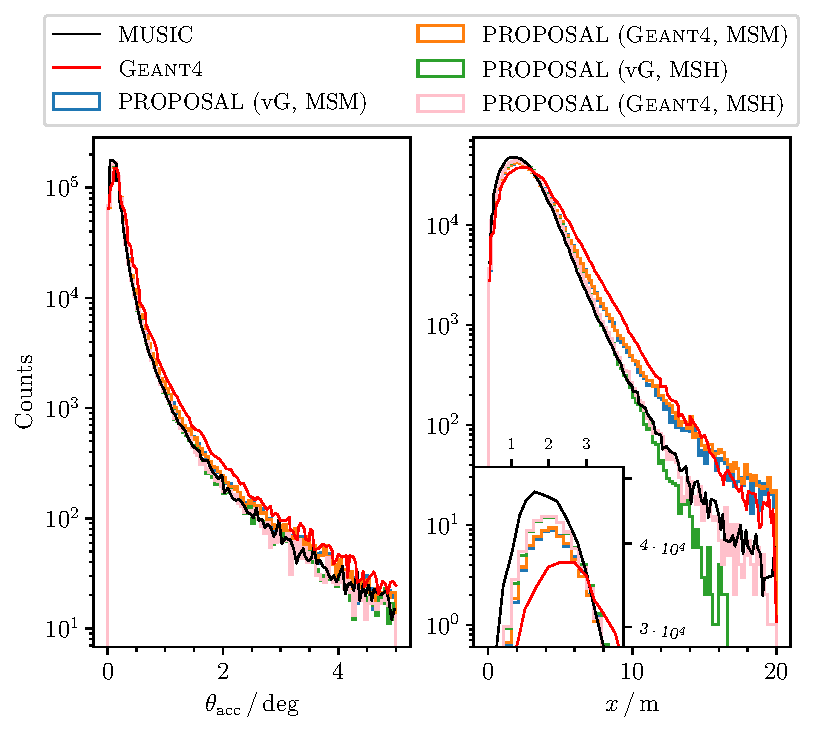
\includegraphics[width=0.43\textwidth]{img/2TeV_1e6events_accumulated_defl_paper_combined_zoom.pdf}
  \end{multicols*}
  \end{sectionbox*}

% ========================================================================================
% ...formatting examples

% ----------------------------------------------------------------------------------------
%	 Getting Started
% ----------------------------------------------------------------------------------------





% ----------------------------------------------------------------------------------------
%  Colors 1)
% ----------------------------------------------------------------------------------------
\begin{sectionbox*}{Good Data-MC Agreements}
  Muon deflection measurements are performed by Attwood for 
    muons propagated with energies of 199\,MeV through 
    109\,mm liquid hydrogen and by Akimenko for muons 
    propagated with energies of 7.3\,GeV through 
    1.44\,cm copper. The deflections simulated with PROPOSAL are in good agreement with the data.
  \begin{multicols*}{2}
    \raggedright
    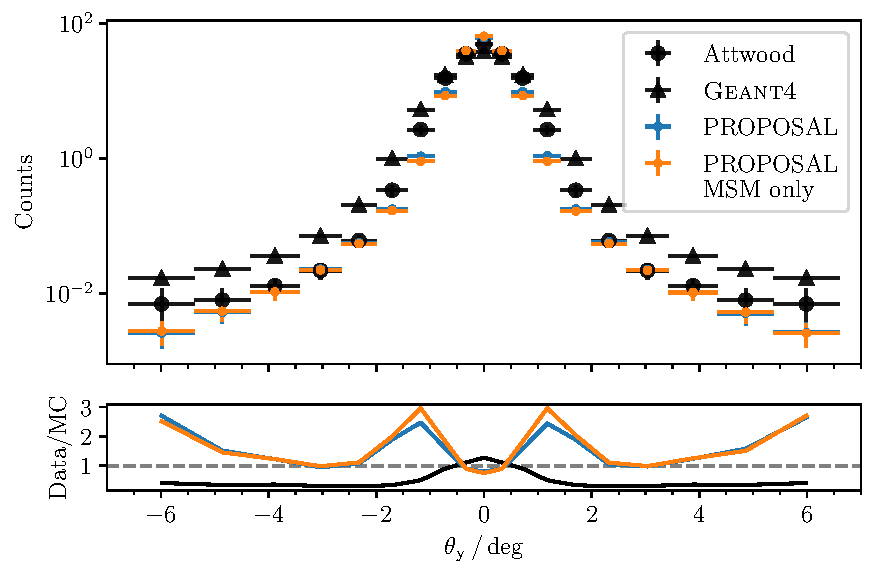
\includegraphics[width=0.44\textwidth]{img/attwood_comparison_moliere_199MeV_final_multi_mean_deg_ratio.pdf}
    \columnbreak
    \raggedleft
    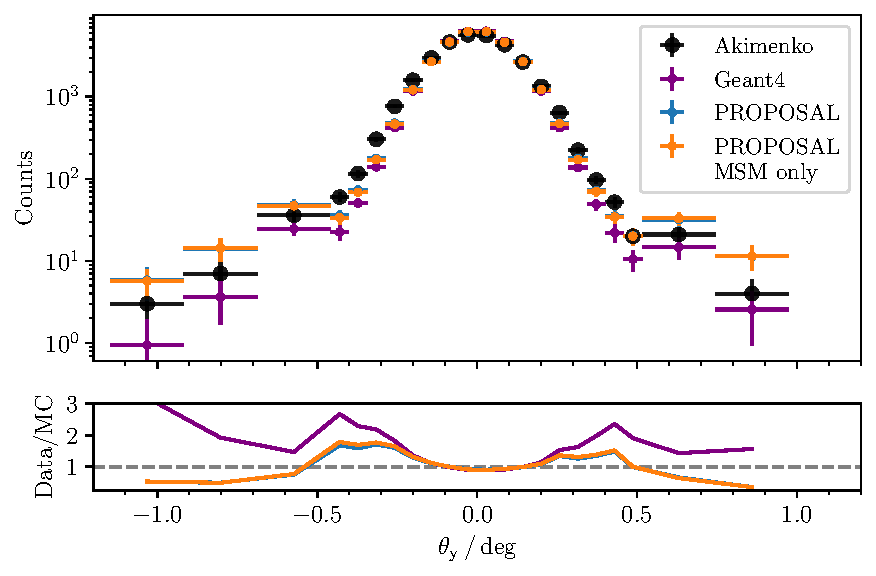
\includegraphics[width=0.44\textwidth]{img/akimenko_comparison_moliere_E7301MeV_final_multi_mean_deg_ratio_G4_v1_final_n100.pdf}
  \end{multicols*}
\end{sectionbox*}

\begin{sectionbox*}{Muon Deflection Impact on Current Experiments}
  \begin{multicols*}{2}
    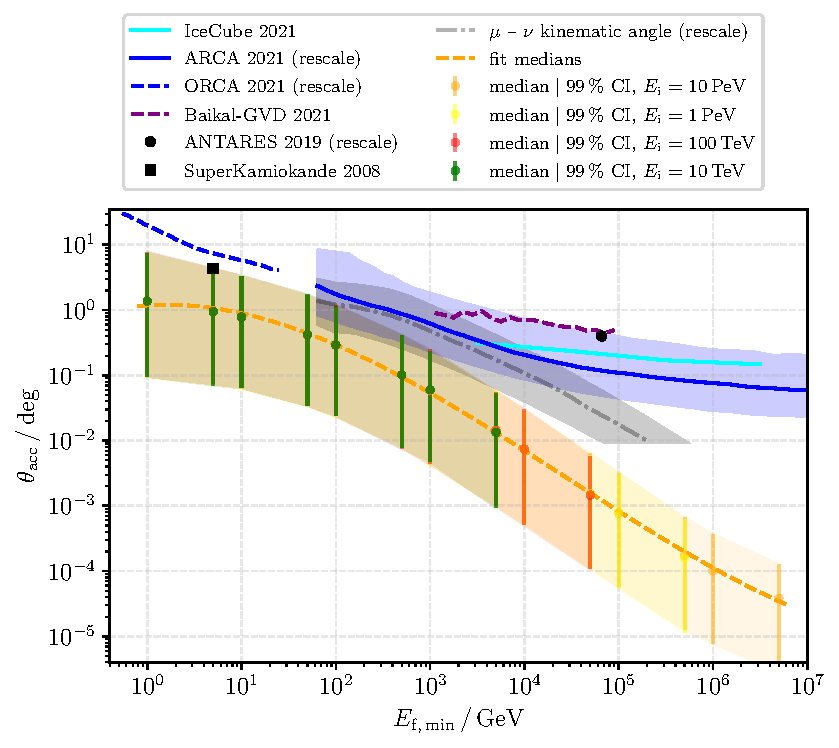
\includegraphics[width=0.44\textwidth]{img/fit_median_defl_cut_10percent_only_poly_new_resolution_rescale_no_icecube_paper_final_all.pdf}
    \columnbreak
    \FloatBarrier
    Muons are propagated through ice with several initial energies to different final energies. 
    The lower the final energy, the larger the muon deflection. Since the medians overlap for different initial energies, 
    the total muon deflection is 
    nearly independent of the initial energy. Thus the muon energy reconstructed at the detector entry can be used to estimate 
    the muon deflection before the entry. 
    
    All medians are fitted by a polynomial which can be used to estimate the muon deflection as a function of the final muon energy. 
    The function can be found in Ref.~\cite{muon_deflection}.
    (The deviations of the muon deflection for a propagation in water are less than 1\,\% for all energies.) 
  \end{multicols*}
\end{sectionbox*}


\end{minipage}


% \noindent
% \begin{minipage}[t][515mm][t]{1\columnwidth} % {\columnwidth}, height: 875mm
% \raggedright
% ----------------------------------------------------------------------------------------
%  Colors 2)
% ----------------------------------------------------------------------------------------
% \begin{sectionbox}[tu03]{Colors}
%   A pre-defined color palette consists of \texttt{tu01}--\texttt{tu11}, each of which
%   has the variations \texttt{tuXXlight}, \texttt{tuXXmidlight}, \texttt{tuXXmiddark}, and
%   \texttt{tuXXdark}.

%   The default color is \texttt{tu01}, above you can see \texttt{tu02}, and this here very
%   box is set to \texttt{tu03}.
% \end{sectionbox}

% \begin{sectionbox*}{\texttt{Example: sectionbox*}}
%   This is a \,\texttt{sectionbox*}\, environment.

%   The star defines that no \,\texttt{\textbackslash vfill}\, is inserted after the box, i.e.
%   the next box comes directly after this one.
% \end{sectionbox*}


% \begin{plainbox*}
%   \begin{center}
%     \Large This is a \,\texttt{plainbox}\, environment
%   \end{center}
% \end{plainbox*}

% \begin{infobox}
%   This is an \,\texttt{infobox}\, environment, floated to the bottom because the previous box
%   did not use a star variant of \,\texttt{plainbox}\,.
% \end{infobox}

% ========================================================================================

% column break
% \end{minipage}
% \columnbreak

\noindent
\begin{minipage}[t][875mm][t]{\columnwidth}
\centering

% \begin{plainbox*}
% \end{plainbox*}
% \hspace{415mm}


% \begin{sectionbox}[tu04]{Resource constraints}
%   What are the resource constraints of your methods/algorithms/application?
%   Which constraints apply to the hardware you are using?
% \end{sectionbox}



% ========================================================================================
% ...formatting example

% \begin{plainbox*}
%   Below you see the result of the command \texttt{\textbackslash maketakeawaybox},
%   where you can hang DIN A4 printouts of your poster.

%   This note has been set up with a \,\texttt{plainbox*}\, environment.
% \end{plainbox*}


% ----------------------------------------------------------------------------------------
%  Takeaway Box
% ----------------------------------------------------------------------------------------
% \maketakeawaybox
% ========================================================================================


% column break
\end{minipage}
\columnbreak

\noindent
\begin{minipage}[t][875mm][t]{\columnwidth}
\raggedleft

% ----------------------------------------------------------------------------------------
%  Results
% ----------------------------------------------------------------------------------------






% ----------------------------------------------------------------------------------------
%  Conclusion and Outlook
% ----------------------------------------------------------------------------------------

% \begin{sectionbox}{Propagation Distance and Unknown Initial Energy}
%   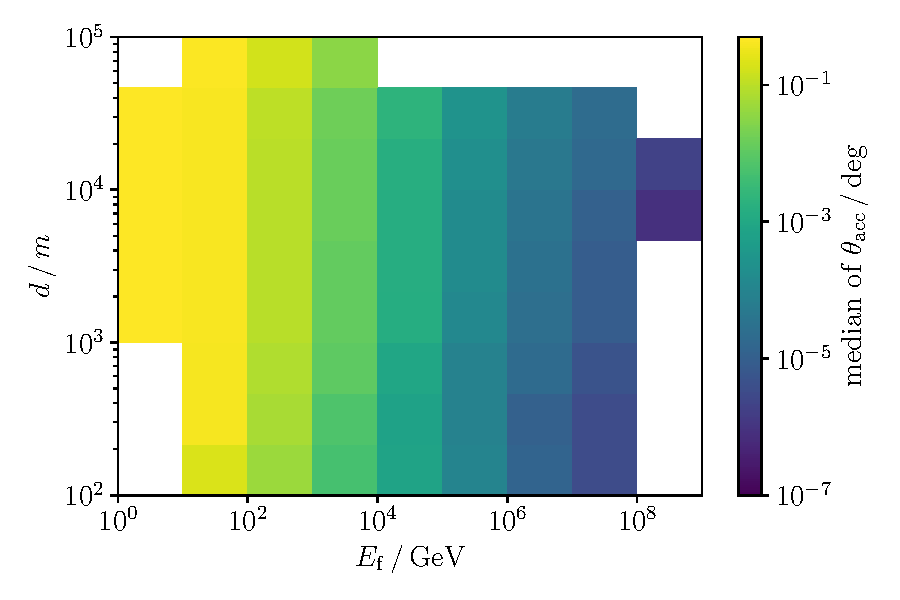
\includegraphics[width=0.44\textwidth]{img/gaisserE37_median_paper.pdf}
% \end{sectionbox}

\begin{sectionbox}{Relevance for Muography}
  Muography is a technique to analyze the inner structures of vulcanoes, pyramids, mines and much more.
  Muons produced in the atmosphere are measured and due to different densities, the muon flux 
  differentiates in front of and behind an object. The angular resolution of these detectors is 
  about 0.6\,°, wich is on the order of magnitude of the muon deflection at GeV energies. 
\end{sectionbox}

\begin{sectionbox}{Conclusion}
  Muon deflections simulated with the propagation tool PROPOSAL are in good agreement with common simulation 
  tools MUSIC and \textsc{Geant4} and two measurements. 
  For muon energies below 3\,TeV, the muon deflection is 
  on the same order of magnitude as the kinematic scattering angle between 
  the incoming neutrino and the produced muon. In comparison with angular resolutions 
  of current muon detectors, the muon deflections become relevant for energies 
  below 1\,TeV. 
\end{sectionbox}


\begin{sectionbox}{Future Research}
  So far, muon deflections are measured only for energies of 7.3\,GeV and lower.
  To approve the correctness of the simulated muon deflection for higher energies, 
  measurements of muons with energies up to TeV or even PeV are required.
  Furthermore, the muon deflection has to be considered if the angular resolutions 
  increase in future experiments and optimizations. 
\end{sectionbox}



% \begin{sectionbox}[tu03]{PROPOSAL}
\begin{infobox}  
  The lepton propagation tool PROPOSAL is available at 
  \href{github.com/tudo-astroparticlephysics/PROPOSAL}{github.com/tudo-astroparticlephysics/PROPOSAL}.
\end{infobox}
  % \end{sectionbox}

% ----------------------------------------------------------------------------------------
%  References
% ----------------------------------------------------------------------------------------
\begin{plainbox*}
  \nocite{*} % print uncited references
  \bibliographystyle{unsrt} % plain reference style
  \bibliography{\jobname}
  \textit{Note: All figures are taken from Ref.~\cite{muon_deflection}.}
\end{plainbox*}


% ----------------------------------------------------------------------------------------
%  Author Section
% ----------------------------------------------------------------------------------------
\begin{infobox}
  \begin{tikzpicture}
    \node[anchor=north west, outer ysep=4pt, inner sep=0pt]
      (title) at (0pt,0pt) {\bfseries\large Pascal Gutjahr};
    \node[anchor=north east, outer sep=0pt, inner sep=4pt, rectangle, rounded corners=2pt, very thick, draw=black, fill=white]
      (picture) at (\textwidth,0pt) {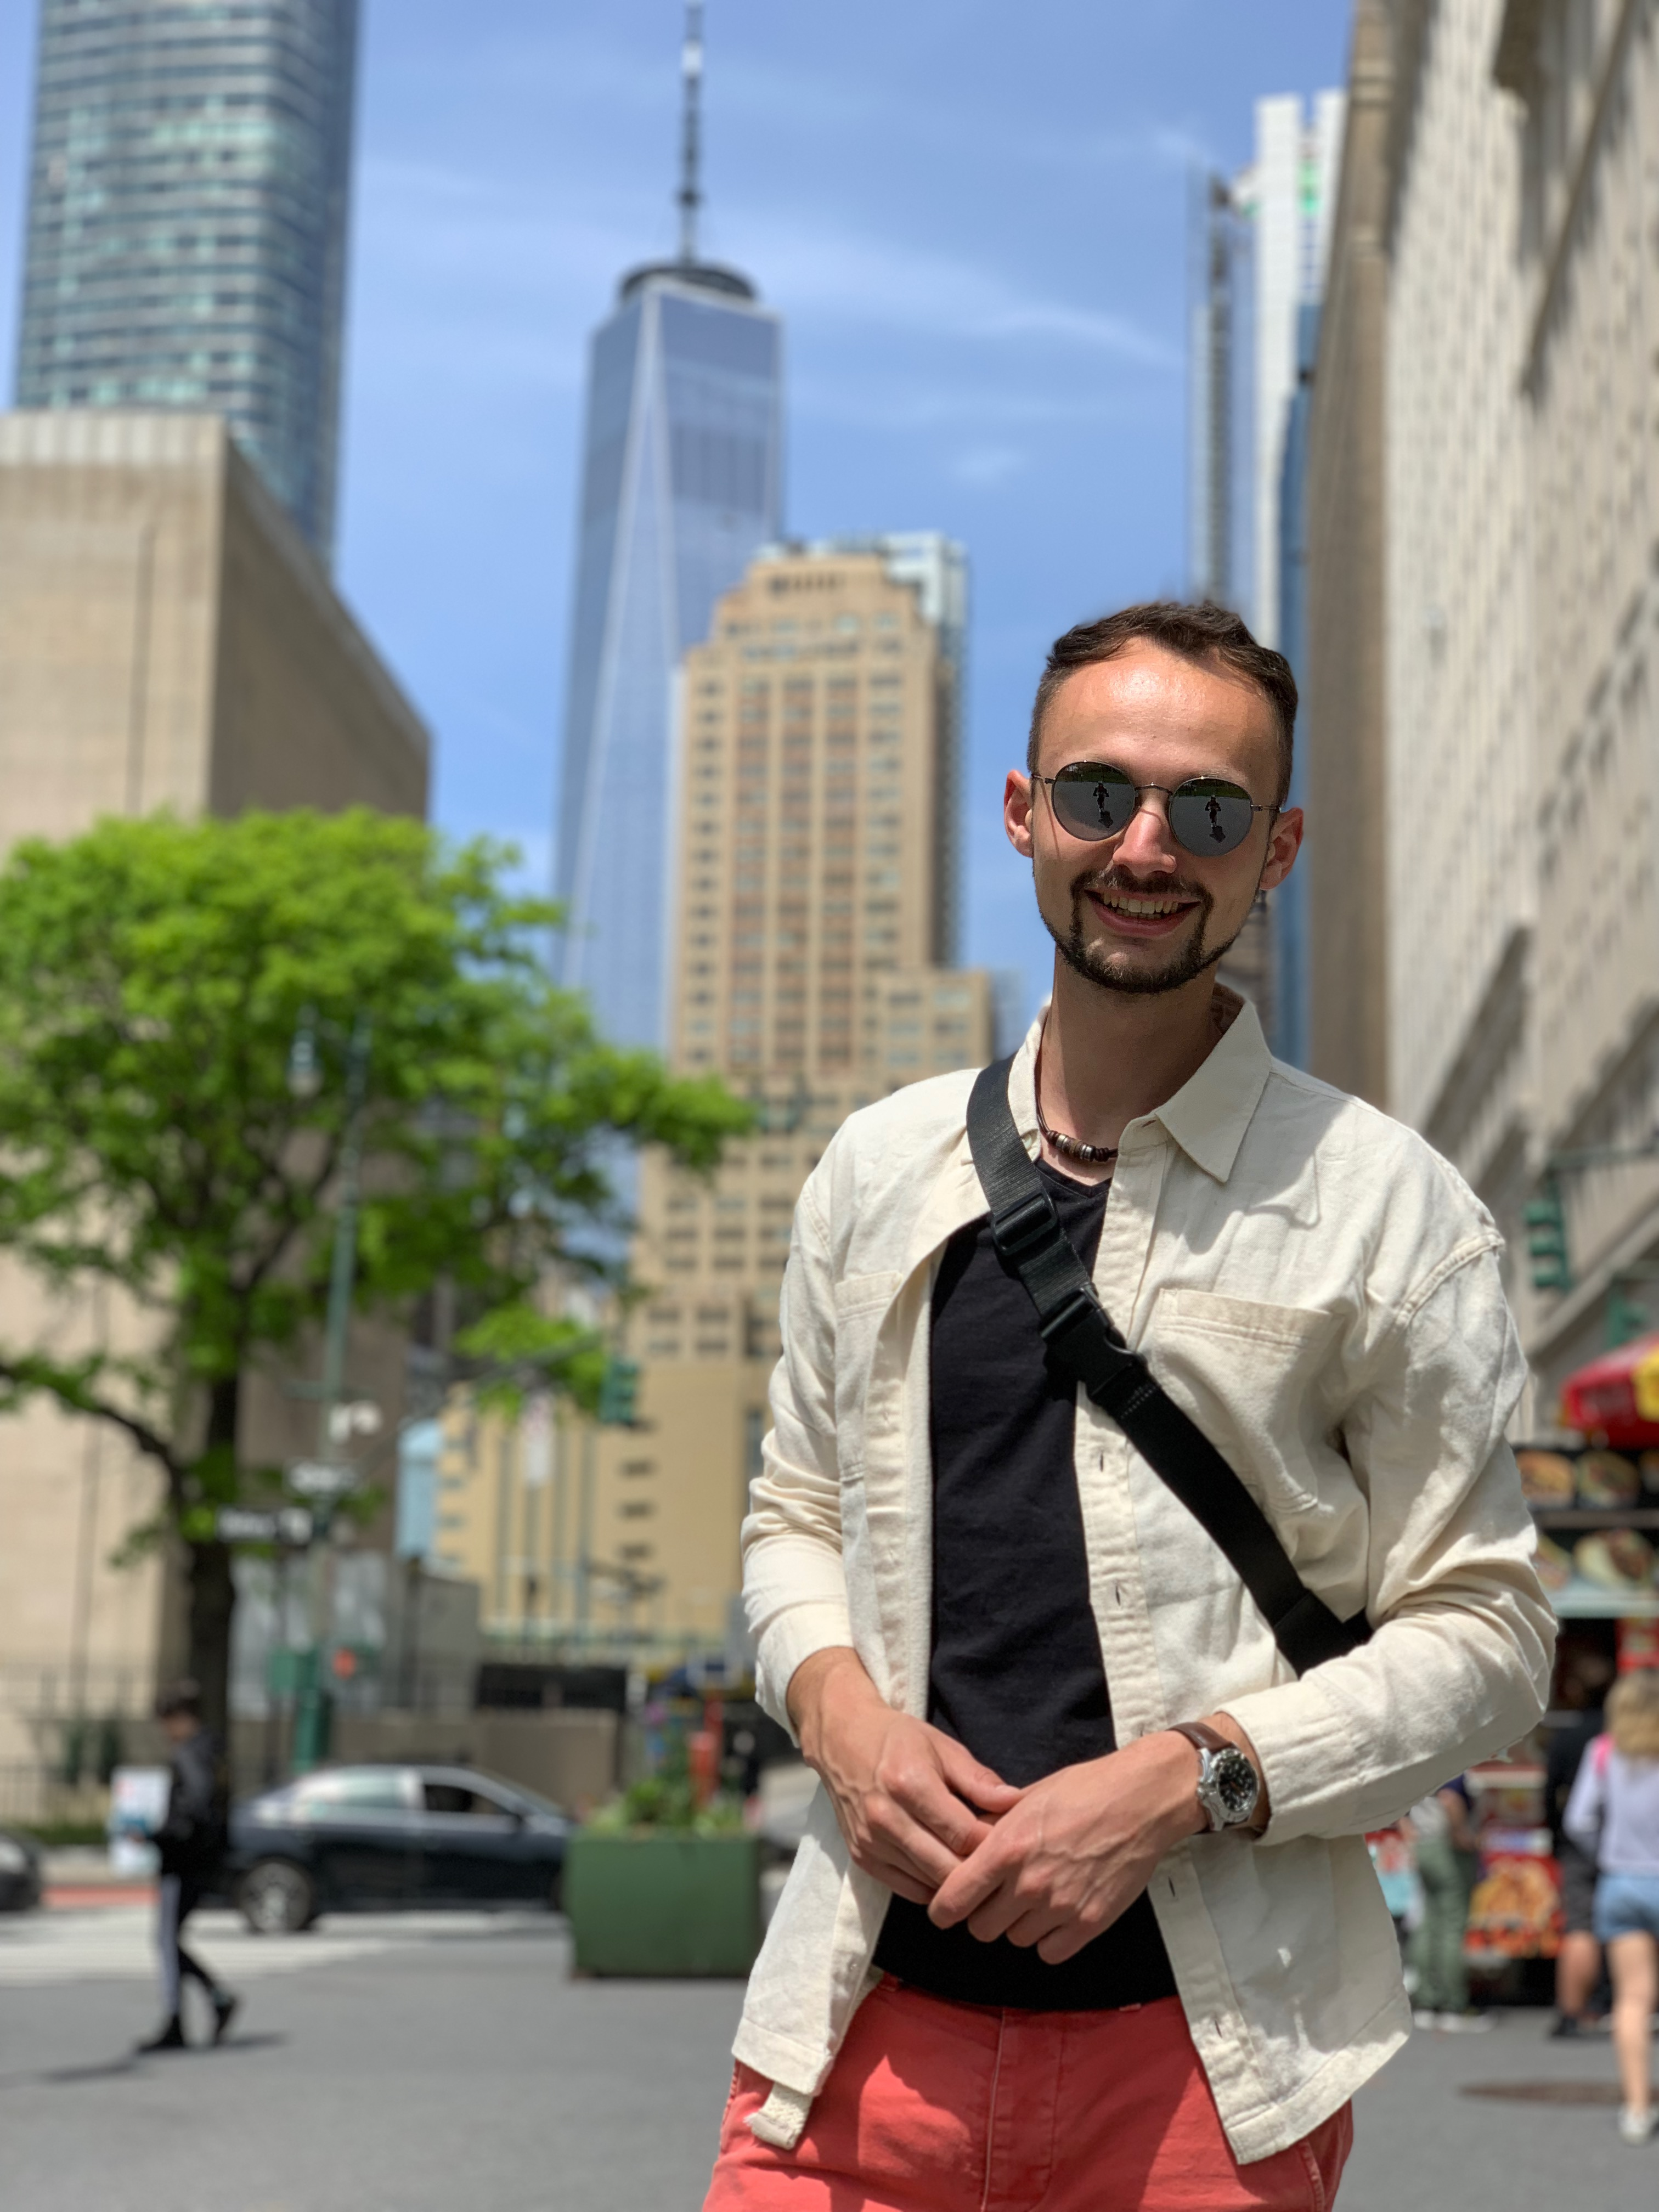
\includegraphics[height=75mm]{img/pascal}};

    \node[anchor=north west, outer xsep=0pt, inner xsep=0pt, outer ysep=0mm, text width=.65\textwidth, yshift=-3pt]
      (enumeration) at (title.south west) {%
        \begin{itemize}
          \item PhD student since 2021
          \item PROPOSAL maintainer 
          \item IceCube member 
        \end{itemize}
    };
    \node[anchor=north west, outer xsep=0pt, inner xsep=0pt, outer ysep=1mm, text width=.65\textwidth]
      (text) at (enumeration.south west) {%
        
      };
  \end{tikzpicture}
\end{infobox}
\end{minipage}
% ----------------------------------------------------------------------------------------


\end{multicols*}
\end{document}